\section{Causal analysis \& discovery}
Reconstructing the \textbf{causal relations} behind the phenomena we observe is 
a fundamental problem in all fields of science.
The traditional approach is to conduct active experiments, but in many fields
manipulations of the complex system under study are either impossible, 
unethical, or very expensive.
On the other hand, modern science generates an ever-growing amount of data 
from these systems, in particular time series data.
Concurrently, novel computing hardware today allows efficient processing 
of massive amounts of data. These developments have led to emerging interest 
in the problem of reconstructing causal networks or causal discovery from 
observational time series.\\

The definition of causality is that $X \rightarrow Y$ if and only if an intervention or
manipulation in $X$ has an effect on $Y$.
A practical example could be the altitude and the temperature as in Figure \ref{fig:tempvsheight}.
As the height increases the temperature lowers.

\begin{minipage}[c]{0.3\textwidth}
    \begin{figure}[H]
        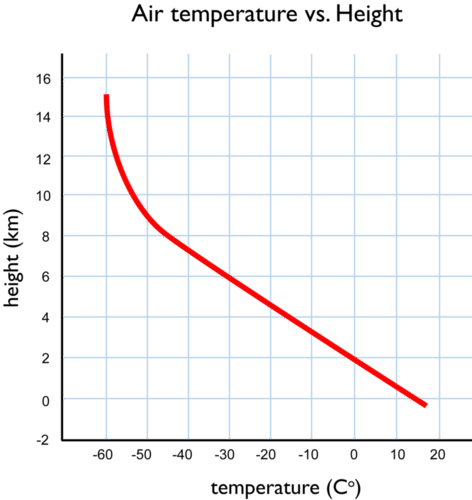
\includegraphics[width=0.6\textwidth]{img/tempvsheight.png}
        \centering
        \caption{Varion of temperature with respect to the height}
        \label{fig:tempvsheight}
    \end{figure}
\end{minipage}
\begin{minipage}[c]{0.6\textwidth}
    One of the main motivations behind causal analysis is a property called \textbf{similability}, 
    the ability o easily predict the output, given only any possible input.
\end{minipage}\\


We will consider causal analysis and discovery for time series since typically, 
input and output of a system are temporal signals, and we are interested in understanding 
how the system evolves and behaves over time.
This means, we want to understand how the temporal evolution of the output signal is affected
by the input signal (\textbf{and discovering which one is the input}).
We will denote as $V_T$ a variable $V$ which is observed for a temporal horizon $T$ (either continuous or
discrete)
\subsection{Structural causal model}
\begin{equation}
    V_t^j \coloneqq \textcolor{red}{f^j}(\textcolor{blue}{pa(V^j_t)}, \eta^j_t)\quad\text{for all }V_t^j\in \bm{V_t} \text{ and } t\in\mathbb{Z}
\end{equation}
Where $\textcolor{red}{f^j}$ is a generic non linear function, $\textcolor{blue}{pa(V^j_t)}$ are the parents of the variable $V^j$ i.e its causes and
$\eta^j_t$ is noise which comes from the uncertanty of the model or of the measurements.
\subsection{Granger's definition of causality (1969)}
Given (temporal) variables $X$ and $Y$, we say that $X\;Granger-causes\;Y$
if $X$ contains information which affects $Y$ at time t, and such
information is not contained in the past of the universe ($Y$'s past or
other variables'past). In other words $Y$ depens \textbf{only} on $X$ and no other variables.If we only consider $Y$, we refer to bivariate causality \\

Granger's definition can be written in the following way:
\begin{equation}
    \bm{x_t}=\sum_{\tau=1}^{\tau_{max}}\phi(\tau)\bm{x}_{t-\tau}+\eta_t
\end{equation}
This formulation implies causality in mean (autoregressive model), this 
is a problem since it does not capture information about the distribution of the data.
